\documentclass[tikz,border=5pt]{standalone}
\usepackage[T1]{fontenc}
\usepackage{lmodern}
\usetikzlibrary{arrows.meta,positioning}
\begin{document}
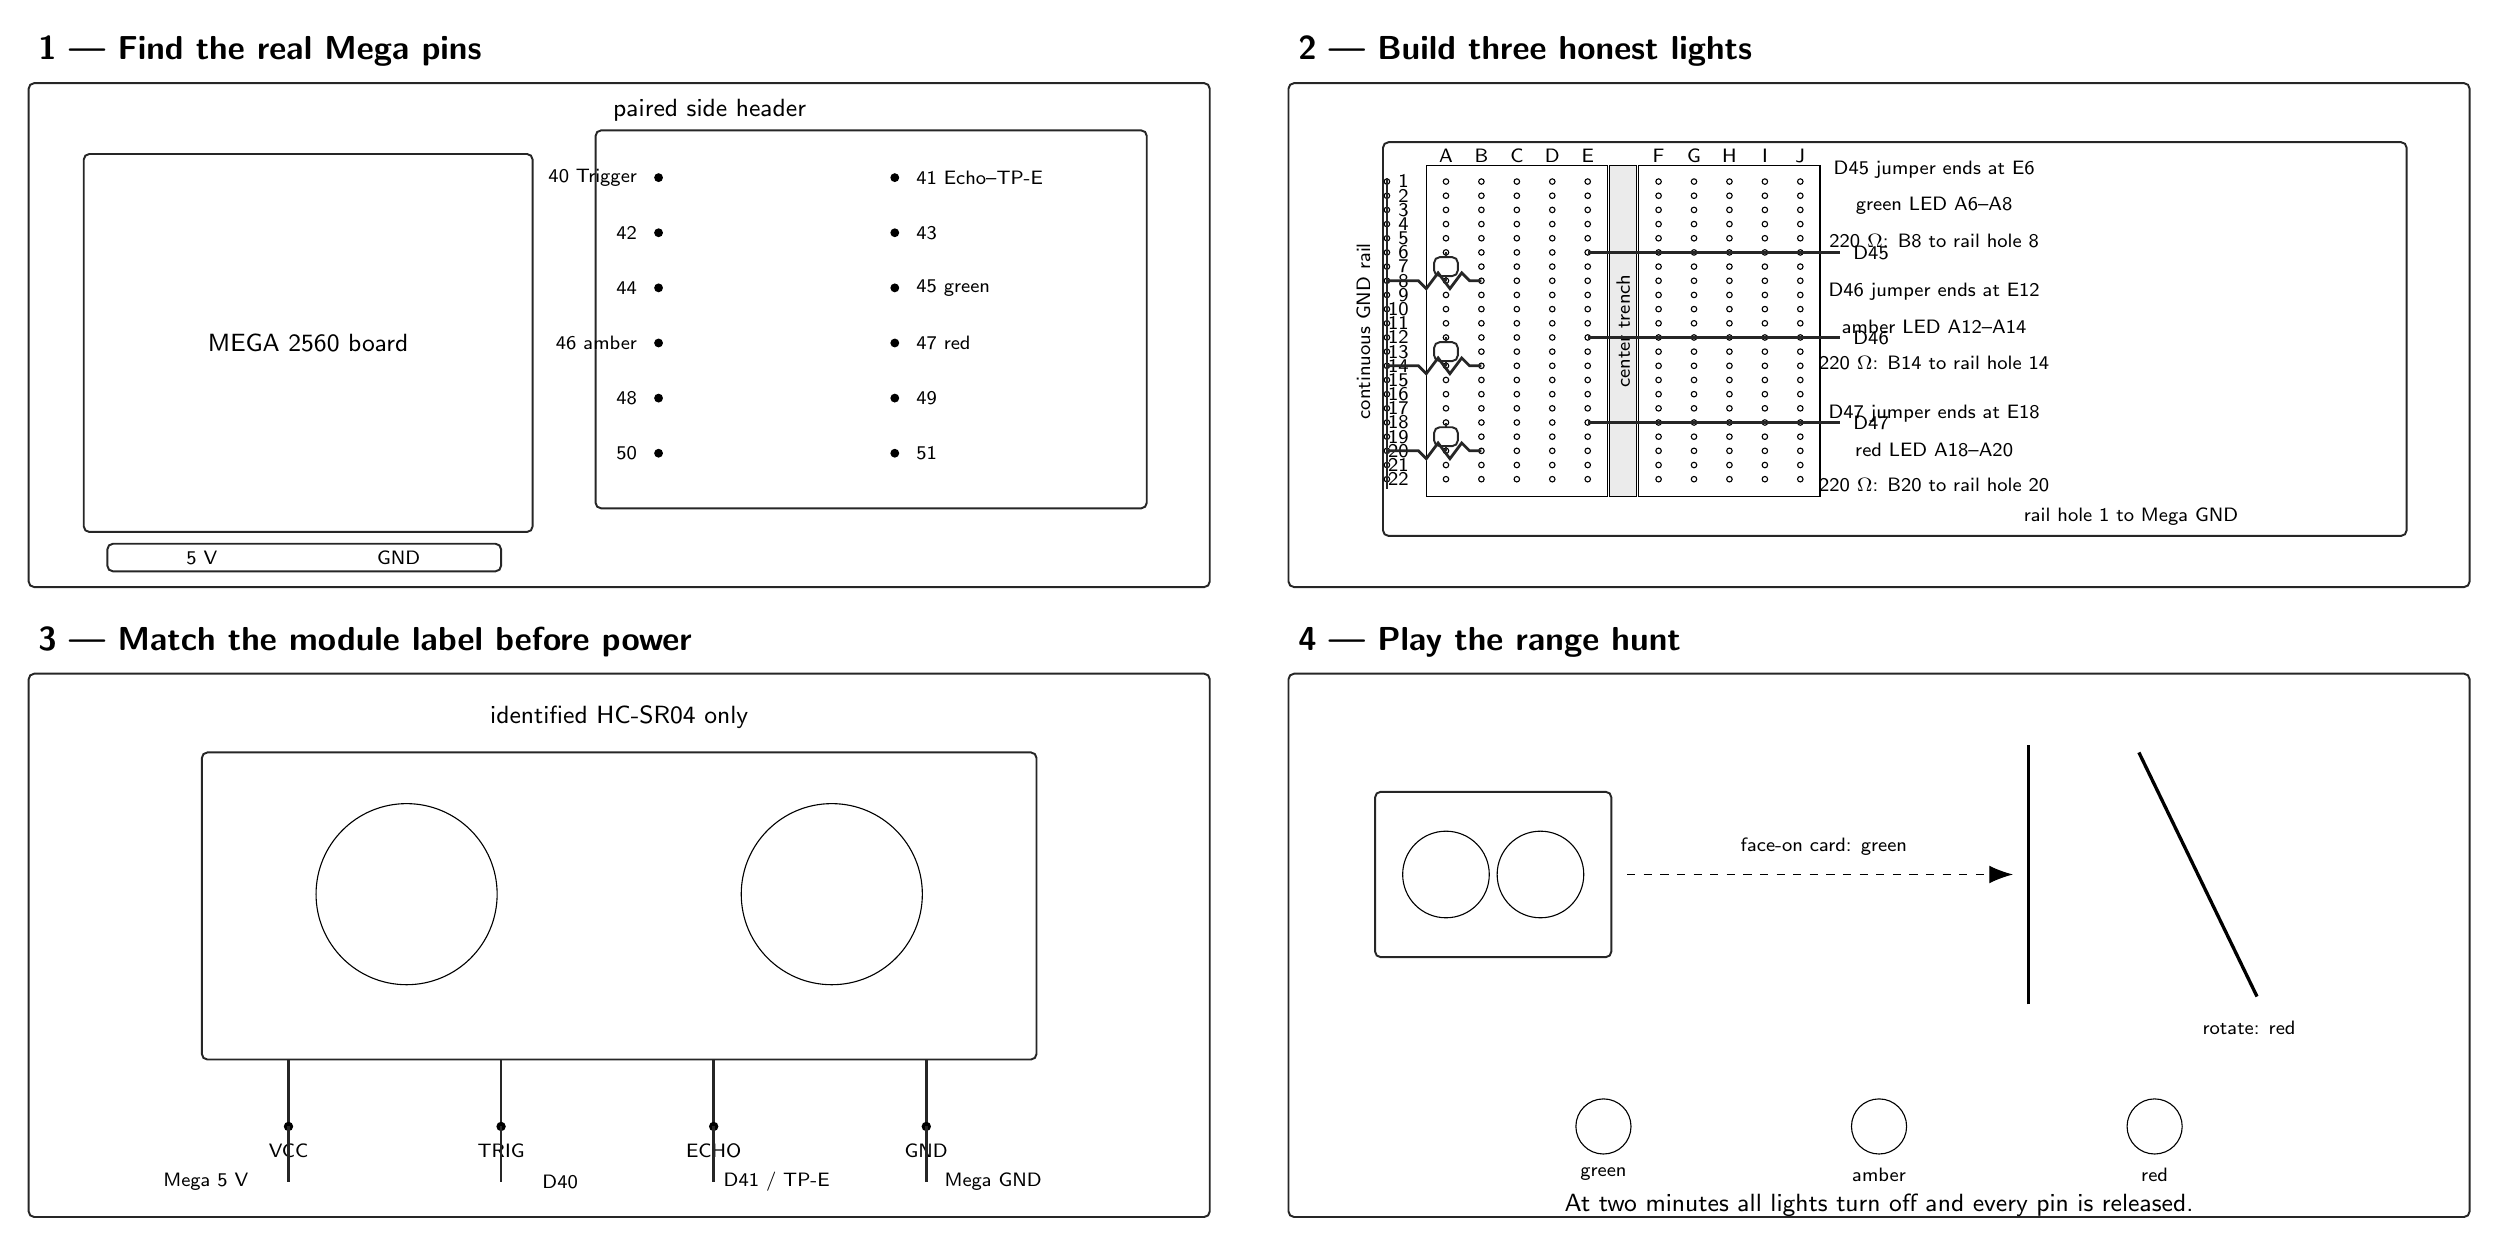
\begin{tikzpicture}[
  x=1cm,y=1cm,
  ink/.style={draw=black!85,line width=.7pt,rounded corners=2pt},
  wire/.style={draw=black!85,line width=1pt},
  note/.style={font=\sffamily\small},
  tinylabel/.style={font=\sffamily\scriptsize},
  title/.style={font=\sffamily\bfseries\large}
]
  \node[title,anchor=west] at (0,14.8) {1 --- Find the real Mega pins};
  \draw[ink] (0,8) rectangle (15,14.4);
  \draw[ink] (0.7,8.7) rectangle (6.4,13.5);
  \node[note] at (3.55,11.1) {MEGA 2560 board};
  \draw[ink] (7.2,9) rectangle (14.2,13.8);
  \node[note,anchor=west] at (7.3,14.05) {paired side header};
  \foreach \y/\left/\right in
    {13.2/40 Trigger/41 Echo--TP-E,12.5/42/43,11.8/44/45 green,
     11.1/46 amber/47 red,10.4/48/49,9.7/50/51}
  {
    \fill (8.0,\y) circle (1.6pt);
    \fill (11.0,\y) circle (1.6pt);
    \node[tinylabel,anchor=east] at (7.85,\y) {\left};
    \node[tinylabel,anchor=west] at (11.15,\y) {\right};
  }
  \draw[ink] (1,8.2) rectangle (6,8.55);
  \node[tinylabel] at (2.2,8.37) {5 V};
  \node[tinylabel] at (4.7,8.37) {GND};

  \node[title,anchor=west] at (16,14.8) {2 --- Build three honest lights};
  \draw[ink] (16,8) rectangle (31,14.4);
  \draw[ink] (17.2,8.65) rectangle (30.2,13.65);
  \draw (17.75,9.15) rectangle (20.05,13.35);
  \draw (20.45,9.15) rectangle (22.75,13.35);
  \draw[fill=black!8] (20.08,9.15) rectangle (20.42,13.35);
  \node[tinylabel,rotate=90] at (20.25,11.25) {center trench};
  \foreach \column/\x in
    {A/18.0,B/18.45,C/18.9,D/19.35,E/19.8,
     F/20.7,G/21.15,H/21.6,I/22.05,J/22.5}
  {
    \node[tinylabel] at (\x,13.48) {\column};
    \foreach \row in {1,...,22}
    {
      \pgfmathsetmacro{\holey}{13.15-(\row-1)*0.18}
      \draw (\x,\holey) circle (.035);
    }
  }
  \foreach \row in {1,...,22}
  {
    \pgfmathsetmacro{\holey}{13.15-(\row-1)*0.18}
    \node[tinylabel,anchor=east] at (17.65,\holey) {\row};
    \draw (17.25,\holey) circle (.035);
  }
  \draw[wire] (17.25,9.25) -- (17.25,13.2);
  \node[tinylabel,rotate=90] at (16.95,11.25) {continuous GND rail};
  \node[tinylabel] at (24.2,13.3) {D45 jumper ends at E6};
  \node[tinylabel] at (24.2,12.85) {green LED A6--A8};
  \node[tinylabel] at (24.2,12.4) {220 \(\Omega\): B8 to rail hole 8};
  \node[tinylabel] at (24.2,11.75) {D46 jumper ends at E12};
  \node[tinylabel] at (24.2,11.3) {amber LED A12--A14};
  \node[tinylabel] at (24.2,10.85) {220 \(\Omega\): B14 to rail hole 14};
  \node[tinylabel] at (24.2,10.2) {D47 jumper ends at E18};
  \node[tinylabel] at (24.2,9.75) {red LED A18--A20};
  \node[tinylabel] at (24.2,9.3) {220 \(\Omega\): B20 to rail hole 20};
  \node[tinylabel] at (26.7,8.9) {rail hole 1 to Mega GND};

  \foreach \pin/\row/\name in {D45/6/green,D46/12/amber,D47/18/red}
  {
    \pgfmathsetmacro{\anodey}{13.15-(\row-1)*0.18}
    \pgfmathsetmacro{\cathodey}{13.15-(\row+1)*0.18}
    \draw[wire] (23.0,\anodey) -- (19.8,\anodey);
    \node[tinylabel,anchor=west] at (23.05,\anodey) {\pin};
    \draw[wire] (18.0,\anodey) -- (18.0,\cathodey);
    \draw[ink,fill=white] (17.85,{(\anodey+\cathodey)/2-.12})
      rectangle (18.15,{(\anodey+\cathodey)/2+.12});
    \draw[wire] (18.45,\cathodey) -- (18.3,\cathodey)
      -- ++(-.1,.10) -- ++(-.15,-.20) -- ++(-.15,.20)
      -- ++(-.15,-.20) -- ++(-.1,.10) -- (17.25,\cathodey);
  }

  \node[title,anchor=west] at (0,7.3) {3 --- Match the module label before power};
  \draw[ink] (0,0) rectangle (15,6.9);
  \draw[ink] (2.2,2.0) rectangle (12.8,5.9);
  \draw (4.8,4.1) circle (1.15);
  \draw (10.2,4.1) circle (1.15);
  \node[note] at (7.5,6.35) {identified HC-SR04 only};
  \foreach \x/\name in {3.3/VCC,6.0/TRIG,8.7/ECHO,11.4/GND}
  {
    \draw[wire] (\x,2.0) -- (\x,1.15);
    \fill (\x,1.15) circle (1.7pt);
    \node[tinylabel,below] at (\x,1.05) {\name};
  }
  \node[tinylabel] at (2.25,.45) {Mega 5 V};
  \draw[wire] (3.3,1.15) -- (3.3,.45);
  \node[tinylabel] at (6.75,.45) {D40};
  \draw[wire] (6,1.15) -- (6,.45);
  \node[tinylabel] at (9.5,.45) {D41 / TP-E};
  \draw[wire] (8.7,1.15) -- (8.7,.45);
  \node[tinylabel] at (12.25,.45) {Mega GND};
  \draw[wire] (11.4,1.15) -- (11.4,.45);

  \node[title,anchor=west] at (16,7.3) {4 --- Play the range hunt};
  \draw[ink] (16,0) rectangle (31,6.9);
  \draw[ink] (17.1,3.3) rectangle (20.1,5.4);
  \draw (18,4.35) circle (.55);
  \draw (19.2,4.35) circle (.55);
  \draw[dashed,-{Latex[length=3mm]}] (20.3,4.35) -- (25.2,4.35);
  \draw[line width=1.2pt] (25.4,2.7) -- (25.4,6);
  \node[tinylabel] at (22.8,4.7) {face-on card: green};
  \draw[line width=1.2pt] (28.3,2.8) -- (26.8,5.9);
  \node[tinylabel] at (28.2,2.4) {rotate: red};
  \foreach \x/\name in {20/green,23.5/amber,27/red}
  {
    \draw (\x,1.15) circle (.35);
    \node[tinylabel,below] at (\x,.75) {\name};
  }
  \node[note] at (23.5,.15)
    {At two minutes all lights turn off and every pin is released.};
\end{tikzpicture}
\end{document}
